\documentclass[UTF8]{ctexart}
\usepackage{graphicx}
\usepackage{cite}
\usepackage{enumerate}
\usepackage{geometry}
\title{EI339 Class Project Report}
\author{陈子轩 516030910545}
\date{2018年12月}
\geometry{a4paper}
\begin{document}
\maketitle
\tableofcontents
\section{问题描述}
\subsection{股价变动机制}
\begin{figure}[!htbp]
\centering
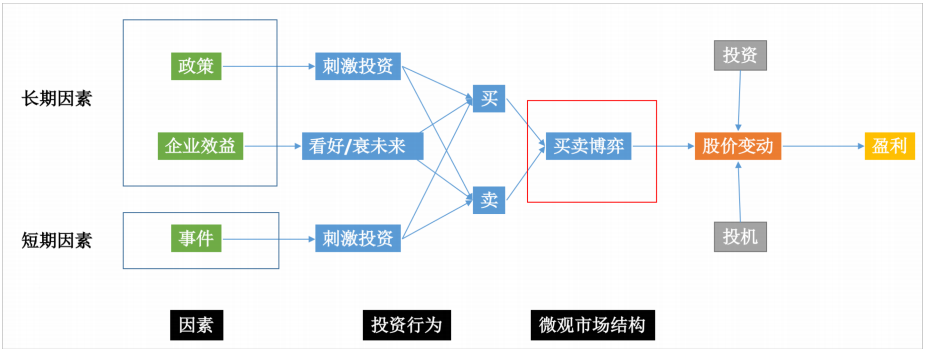
\includegraphics[scale = 0.6]{p1.png}
\caption{股价变动机制}
\end{figure}
如图所示,影响股价变动的机制有长期因素和短期因素,他们都最终归结为买卖博弈来影响价格。买卖博弈可以通过三个方面体现:已公开的买卖需求、正在实施的买卖动作、持币观望。已公开的买卖需求可以通过订单簿来体现,正在实施的买卖动作经研究可以看做是随机尝试的实现,而第三类信息是难以获得的。本次大作业主要研究订单簿对价格的影响。
\subsection{数据描述}
订单簿的数据为:
\begin{enumerate}[*]
    \item 日期(Date)
    \item 时间(Time)
    \item 申买价(Bid Price)
    \item 申买量(Bid Volume)
    \item 申卖价(Ask Price)
    \item 申卖量(Ask Volume)
    \item 最新成交价(Last Price)
    \item 中间价(MidPrice = (Bid Price + Ask Price) / 2)
    \item 当前累计成交数量(Volume)
\end{enumerate}
\subsection{任务要求}
通过对订单簿中数据的学习,预测下20个时间点中间价(mid price)的均值
\section{算法设计}
\subsection{LSTM}
\subsubsection{算法介绍}
LSTM(Long-Short-Term-Memory)是RNN的一种变体,要了解LSTM,首先需要了解RNN的工作原理,如下图
\begin{figure}[!htbp]
\centering
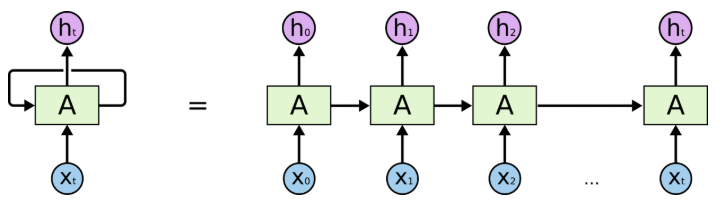
\includegraphics[scale = 0.8]{p3.png}
\caption{Recurrent Neural Network(RNN)\cite{1}}
\end{figure}
\paragraph*{RNN的结构}
传统的RNN包含一个循环态,如图2左边的单元,它可以读入一个输入$x_t$,输出一个$h_t$,从而将状态转移到下一个时间点。如果将这个单元按照时间序列展开则可以得到图二右边的单元序列。由于它的链式的特征,他自然与时间序列和列表产生关联,从而可以解决由于时间的推移所带来的问题。RNN可以利用对先前信息的理解对后续的事件做出预测,例如我们想要预测"the clouds are in the sky"这句话的最后一个单词, 由于根据前面的句子很显然最后一个词就是sky,所以通过RNN可以准确的预测出来。
\paragraph*{RNN的缺陷}
但是如果我们想要预测“I was born in Japan, .... I speak Japanese"这样需要跨越较长的时间序列才能获得的信息时则显得力不从心,这是基于RNN自身结构的问题,但是幸运的是, LSTM并不存在这样的问题。
\paragraph*{LSTM的结构}
LSTM在RNN的基础上,改进了工作单元的机构,传统的RNN模块包含的是重复单一的层,但是LSTM的重复模块包含的是四个交互的层。如下图
\begin{figure}[!htbp]
    \centering
    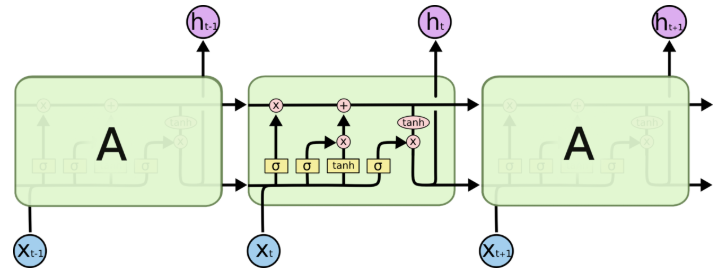
\includegraphics[scale = 0.8]{p4.png}
    \caption{LSTM的重复模块\cite{1}}
\end{figure}
我们将结合图5更进一步介绍LSTM的内部信息。
\begin{figure}[!htbp]
    \centering
    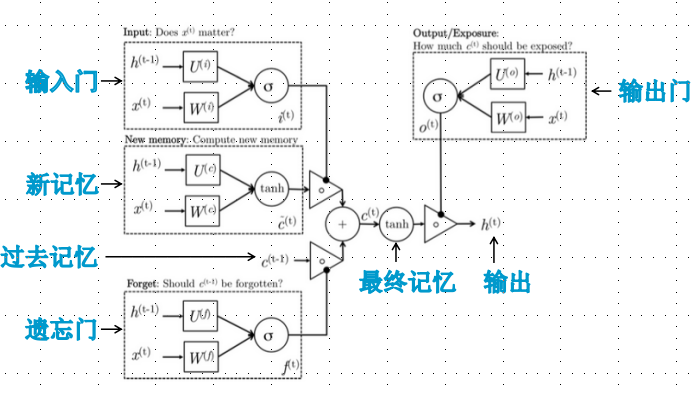
\includegraphics[scale = 0.8]{p5.png}
    \caption{LSTM的内部结构\cite{2}}
\end{figure}
\paragraph*{1. 决定丢弃信息}对于上一个时间点的信息,首先决定丢弃那些信息,这一步通过遗忘门来决定,该门将读取$h_{t-1}$和$x_t$,输出一个$f_t$,$f_t$内的值为$[0,1]$,0表示完全舍弃,1表示完全保留。
$$f_t = \sigma(W_f\cdot x_t + U_f\cdot h_{t-1} + b_f)$$
\paragraph*{2. 确定新信息}
下一步将是决定什么样的新信息将被存放在细胞状态中,这一步包含两个门,输入门和新记忆,\textbf{新记忆}通过tanh函数构建候选信息向量,\textbf{输入门}通过sigmoid函数判定什么值将要更新。
$$i_t = \sigma(W_i\cdot x_t + U_i\cdot h_{t-1} + b_f)$$
$$a_t = \sigma(W_a\cdot x_t + U_a\cdot h_{t-1} + b_f)$$
\paragraph*{3. 更新细胞状态}
然后,新记忆将于旧记忆结合构成新的细胞状态
$$C_t = f_t\cdot C_{t-1} + i_t \cdot a_t$$
\paragraph*{4. 确定新信息}
最后,我们通过一个\textbf{输出门}决定什么将被输出
$$o_t = \sigma(W_o\cdot x_t + U_o\cdot h_{t-1} + b_f)$$
$$h_t = tanh(C_t)\cdot o_t$$
\subsubsection{建模方式}
\begin{figure}[!htbp]
    \centering
    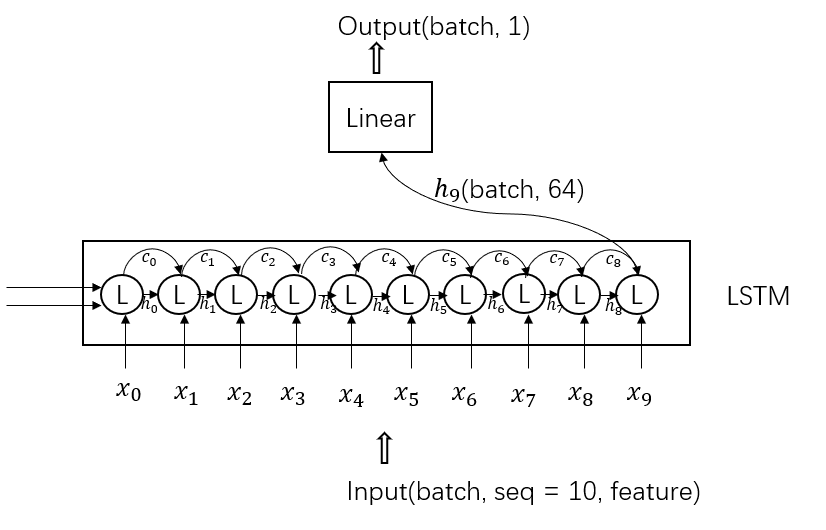
\includegraphics[scale = 0.6]{p6.png}
    \caption{LSTM建模\cite{2}}
\end{figure}
如图5,根据LSTM的模型特征,我们选择通过前10天的订单簿数据预测下20个时间点中间价(mid price)的均值,即时间序列长度seq = 10。选择的输入特征为订单簿的各类数据,包括['MidPrice', 'LastPrice', 'Volume', 'BidPrice1', 'BidVolume1', 'AskPrice1', 'AskVolume1', 'VolDiff'],其中VolDiff由相邻两日的Volume之差组成

\subsubsection{参数选择依据}
\subsection{DNN}
\subsubsection{算法介绍}
\subsubsection{建模方式}
\subsection{其他的尝试——底层LSTM的实现}
由于前面两种模型都是使用pytorch进行搭建的,很多内部结构以及前向传播和反向传播过程都是由pytorch内部自动完成的,为了进一步探究关于LSTM的内部数据传递和前向和反向传递的原理,我们使用numpy从底层对LSTM进行了实现。
\subsubsection{模型搭建的方法}
如果需要从底层实现LSTM,则需要掌握它的前向传播和反向传播的原理,前向传播参考LSTM模型介绍。一下重点介绍反向传播。
\subsubsection{建模方式}
\begin{figure}[!htbp]
    \centering
    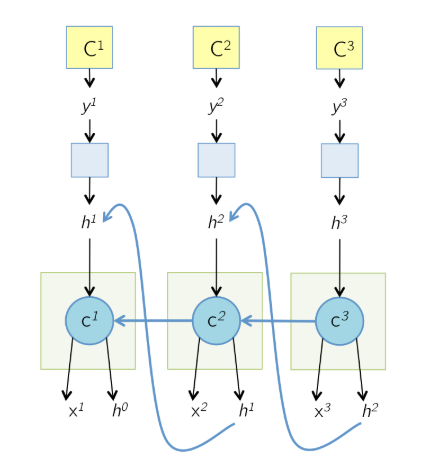
\includegraphics[scale = 0.6]{p7.png}
    \caption{LSTM建模\cite{2}}
\end{figure}
\section{组员分工}
\begin{enumerate}
    \item 陈子轩 LSTM模型搭建,底层LSTM实现,实验报告撰写
    \item 孟令佳 原始数据处理,DNN模型搭建与调参,LSTM模型调参,实验报告撰写
\end{enumerate}
\section{感想}
\paragraph*{}
通过本次大作业,我深刻了解了LSTM模型的原理以及用它来解决实际问题的方法,并且根据自己的理解手动实现了LSTM的前向和反向传播,这让我对于深度学习有了更为深刻的认知,同时也让我体会到了数学基础对于高级算法的决定性作用。同时,在利用深度学习解决实际问题的过程中,我掌握了归一化等数据处理的方式,同时在消除过拟合的解决中学会了使用交叉验证集和正则化的方法,这些技巧对我今后的实践都有很大的帮助。此外,大作业还锻炼了我的耐性,在多次调试仍然效果不好的情况下能够继续耐住性子尝试新的方法,这对我以后都有很大的帮助。最后我想感谢我的队友和同学们,他们在我遇到困难时耐心指导,帮了我很多。最后感谢助教的辛苦工作,让我们能够顺利完成这次作业。

\begin{thebibliography}{3}
    \bibitem{1}https://colah.github.io/posts/2015-08-Understanding-LSTMs/
    \bibitem{2}https://blog.csdn.net/u012319493/article/details/52802302
    \bibitem{3}
    
\end{thebibliography}
\end{document}